\documentclass[runningheads]{llncs}

\usepackage{amssymb,amsmath,mathtools,empheq,fancybox}

\usepackage{paralist}
\usepackage{url}
\usepackage{color}

\usepackage{textcomp,listings}
\usepackage{biblatex}
\usepackage{mymacros}
\usepackage{mathpartir}
\usepackage{csquotes}
\usepackage[font={small,it}]{caption}
\addbibresource{../bibliography.bib}



\newif\ifcomments
\commentstrue

\newcommand{\pr}[1]{{\color{red}``PR: #1''}}
\newcommand{\as}[1]{{\color{blue}``AS: #1''}}

\newif\ifoutline
\outlinetrue

\newcommand{\contents}[1]{\ifoutline{\color{blue}
    \begin{itemize}
    #1
    \end{itemize}
  }\fi}

\allowdisplaybreaks[1]
\title{A Solver for Generalised Parikh Images of Regular Languages}
\author{Philipp Rümmer \& Amanda Stjerna}
\institute{Uppsala University, Sweden}

\begin{document}
\maketitle

\section{Introduction}

Parikh images appears naturally as part of many operations in model checking or
solving of string constraints in automata-based string solvers such as
\Ostrich{} \cite{ostrich}. While it is possible to compute the Parikh image of
an automaton using the method described in \cite{generate-parikh-image}, this
method produces clauses with many existentially quantified variables which are
costly to eliminate, in practice making many real-world applications
intractable. Furthermore, many applications require automata with symbolic
labels to handle large alphabets like Unicode which would increase the number of
variables even more. Finally, automata-based string solvers compute Parikh
images on products of automata, derived from conjunctions of string constraints.
Using \cite{generate-parikh-image} this would require the up-front computation
of the product before its Parikh image, running the risk of an exponential
blow-up.

Addressing these concerns, our approach allows us to extend the computation of
Parikh images to handle symbolic transition labels ergonomically, while also
allowing us to interleave the computations of the Parikh image of a product and
the product itself. This allows both calculations to inform each other, thereby
eliminating unneccesary work. Moreover, the scheme allows us to learn
interesting facts (in the form of implied clauses) about the problem.

Based on these insights, we present a work-in-progress tool to solve linear
constraints on symbolic automata with counters, amounting to constraints on the
Parikh image of their product. We are able to generate symbolic (\enquote{there are
twice as many \texttt{a}:s as \texttt{b}:s}) as well as concrete Parikh images.

\section{Background}

Formally, the \textit{Parikh map} over a context-free language $\Sigma = \left\{a_1, \ldots, a_k \right\}$ is defined as in \cite{kozen}:

$$
\begin{aligned}
& \psi: \Sigma^* \rightarrow \mathbb{N}^k \\
& \psi(s) = \left[\#a_1(s), \#a_2(s), \ldots, \#a_k(s)\right]
\end{aligned}
$$

That is, $\psi(s)$ is a vector of the number of occurrences of each character in the language for a given string $s$. For example, for  $\Sigma = \left \{ a, b\right\}$, we would have $\psi(abb) = \left[1, 2\right]$.

We define the image of this map, the \textit{Parikh image}, of some subset of the language $A \subseteq \Sigma^*$ as:

$$
\psi(A) = \left\{ \psi(x) | x \in A \right\}
$$

Thus we would have $\psi(\left\{ab, abb\right\}) = \left\{\left[1, 1\right], \left[1, 2\right]\right\}$.

\subsection{Generalised Parikh Images}\label{sec:generalised}

Another way of viewing the Parikh map is as a monoid homomorphism $p:\: \left(\Sigma^*, \cdot, \epsilon \right) \to (\mathbb{Z}^\Sigma, +, \vec{0})$, where $\cdot$ is the string concatenation operation, the objects of the right-hand-side monoid are character counts, and $+$ is standard vector addition. Note that while the left monoid does not commute, the right one does.

This viewpoint enables us to generalise the Parikh map and its image further to arbitrary monoid morphisms $h:\: \Sigma^* \to M$ where $M$ is a commutative monoid. It then follows from the universal mapping property that any such morphism $h$ can also be expressed in terms of the Parikh map, as $h' \circ p$.

A useful example of such a morphism might be computing the length of a string,
which could be recast in terms of the Parikh map by summing the individual
character counts of the vector: $h':\: (\mathbb{Z}^\Sigma, +, \vec{0}) \to
(\mathbb{Z}, +, 0) = \vec{x} \to \sum_{i \in \Sigma} x_i$. This allows us to
apply e.g. arithmetic on register variables to the Parikh image calculus.

\section{Lazy Computation of Parikh Images for Regular Languages}

Starting with the automaton shown to the left in figure~\ref{fig:automaton}, we seek
any value in its Parikh image, i.e. a character count.

\begin{figure}[h]
  \caption{Left to right: the starting automaton, the automaton with its corresponding linear equations, and the solution. Note the replacement of the existentially quantified transition variables with character count constants, and the introduction of a linear equation across the edge for \texttt{d} representing a choice between either an~\texttt{a} or a~\texttt{d}. Transitions with a zero value are not used in the solution.}\label{fig:automaton}
  \begin{minipage}[t]{0.3\textwidth}
    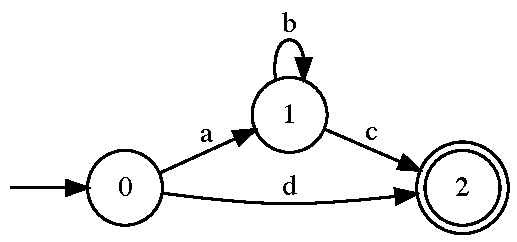
\includegraphics[width=\textwidth]{trace-0}
    \end{minipage}
    \begin{minipage}[t]{0.3\textwidth}
    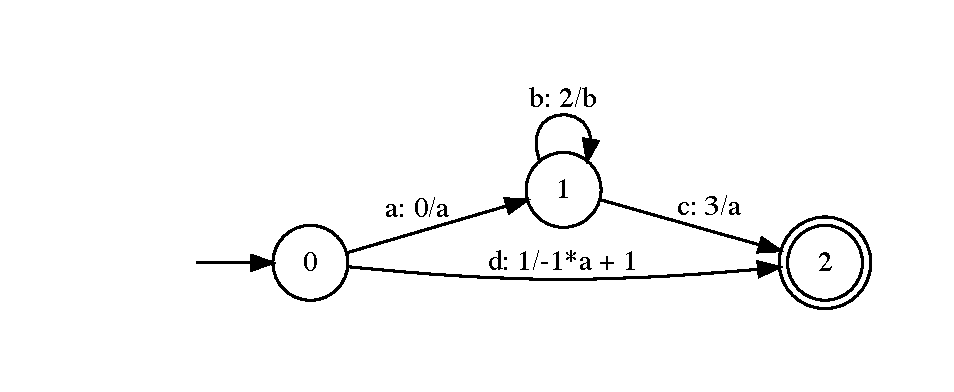
\includegraphics[width=\textwidth]{trace-0-aut-0}
    \end{minipage}
    \begin{minipage}[t]{0.3\textwidth}
      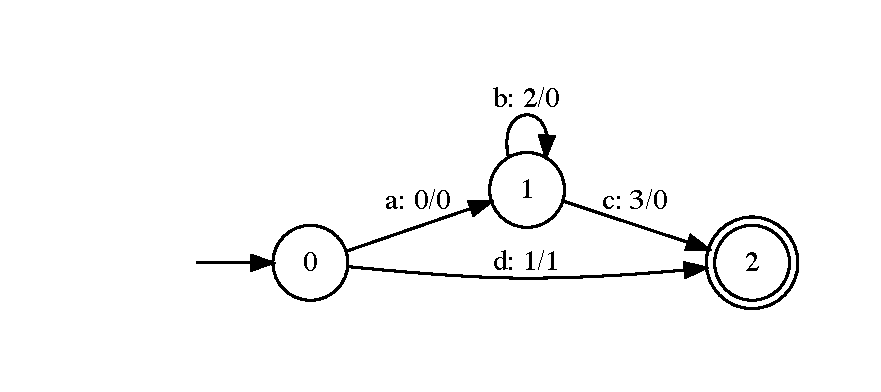
\includegraphics[width=\textwidth]{trace-3-aut-0}
      \end{minipage}
  \end{figure}

  In this case, our calculation will introduce a free integer constant per
  character ($a$, $b$, $c$, and $d$). It will then introduce equations
  preserving flow through the automaton corresponding to how many times that
  transition is used in a run of the automaton. Each transition will be given an existentially
  quantified variable in these equations, and each of our target variables is
  constrained to the sum of the transitions where it occurs as a label. This
  corresponds to the first portion of the formula described
  in~\cite{generate-parikh-image}, but crucially misses the constraints to
  ensure connectedness in the presence of cycles. Instead, we enforce this
  constraint lazily using our own deduction rules.

  Note that this formulation allows us to propagate information between terms of
  a product before materialising it. For many unsatisfiable instances, this
  corresponds to the method recently introduced in~\cite{approximate-parikh},
  where the Parikh image of a product of automata is over-approximated as the
  conjunction of their Parikh images.
  
Before computation using our rules begin, our prover performs reasoning on the flow equations to simplify them into $d + a = 1 \land c = a$.

We now have a choice of two paths for our run and execute a case split: \textsc{Split}: $a \leq 0$ $\mid$ $a > 0$. The split is performed as close to the initial state as possible and favours deselecting an edge by constraining its corresponding term to be 0.

Since this decision disconnects a loop, the $b$~transition, from the initial state, we evaluate the rule \textsc{Propagate-Connected} to add the constraint $b = 0$. Afterwards we can subsume the propagating machinery for the connectedness constraint, as no more loop transitions can be positive. This leaves us with an automaton with just one nonzero transition, as seen in figure~\ref{fig:automaton}.

As there is just one automaton left, there are no products to compute and this the
calculation is complete. We present the solution $a = b = c = 0, d=1$.

%\bibliographystyle{splncs03}
\printbibliography

\end{document}
